\documentclass[a4paper,11pt]{report}
\usepackage[T1]{fontenc}
\usepackage[cp1250]{inputenc}  
\usepackage{amsmath} 
\usepackage{amssymb} 
\usepackage{epsfig} 
\usepackage[a4paper]{geometry} 
\usepackage{cite}
\usepackage{graphicx}
\usepackage{url}
\usepackage{multirow}
\usepackage{array}

\newcommand{\cvut}{Czech Technical University in Prague}
\newcommand{\fjfi}{Faculty of Nuclear Sciences and Physical Engineering}
\newcommand{\km}{Department of Physics}
\newcommand{\obor}{Mathematical Engineering}
\newcommand{\oborcz}{Matematick\'{e} In\v{z}en\'{y}rstv\'{i}}
\newcommand{\zamereni}{Mathematical Physics}

\newcommand{\nazevcz}{Jety s vysokou p\v{r}\'{i}\v{c}nou hybnost\'{i} v RunII experimentu ATLAS}        
\newcommand{\nazeven}{High pT jets in RunII of the ATLAS Experiment}    
\newcommand{\autor}{Jan Lochman}          
\newcommand{\rok}{May 2015}         
\newcommand{\vedouci}{Ing. Zden\v{e}k Hub\'{a}\v{c}ek, Ph.D.}        
\newcommand{\pracovisteVed}{CERN}	

\newcommand{\klicova}{Klicova slova}   
\newcommand{\keyword}{Key words}       

\newcommand{\abstrCZ}{Abstrakt CZ} 
\newcommand{\abstrEN}{Abstrakt EN}                  

\newcommand{\MyQuote}[2]{
  \textit{\quotation{#1}}
  \begin{flushright}
    #2
  \end{flushright}
  \vspace{10mm}
}

\newcolumntype{L}[1]{>{\raggedright\let\newline\\\arraybackslash\hspace{0pt}}m{#1}}
\newcolumntype{C}[1]{>{\centering\let\newline\\\arraybackslash\hspace{0pt}}m{#1}}
\newcolumntype{R}[1]{>{\raggedleft\let\newline\\\arraybackslash\hspace{0pt}}m{#1}}


\begin{document}

%================================================================================
% Titulni stranka
%================================================================================
\thispagestyle{empty}

\begin{center}
    {\Large \textsc{\cvut}\\[1.5ex] \textsc{\fjfi}}\\[1.5ex]{\large \textsc \km}
    \vspace{10mm}

    \begin{tabular}{c}
    {Programme: \obor}\\
    {Branch of Study: \zamereni}
    \end{tabular}

   % logo CVUT -- pokud jej nechcete použít, zakomentujte následující øádek a odkomentujte øádek pod ním:
    \vspace{10mm} \epsfysize=25mm \epsffile{cvut} \epsfysize=25mm \epsffile{fjfi} \vspace{15mm}
   % \vspace{50mm}

   {\huge \bf \nazeven}

   \vspace{15mm}
   {\Large MASTER'S DEGREE PROJECT}

   \vfill
   {\large
    \begin{tabular}{ll}
    Author: & \autor\\
    Supervisor: & \vedouci\\
    Submitted in: & \rok
    \end{tabular}
   }
\end{center}


%================================================================================
% Prazdna stranka
%================================================================================
\newpage  
\thispagestyle{empty} 
~


%================================================================================
% Zadani prace
%================================================================================
\newpage  
\thispagestyle{empty} 
Zadani prace


%================================================================================
% Prohlaseni
%================================================================================
\newpage 
\thispagestyle{empty}  
~
\vfill 
{\bf Statement} 

\vspace{0.5cm} 
Prohlasuji\ldots

\vspace{5mm}V Praze dne ....................\hfill 
............................................       
\begin{flushright}
  \autor 
\end{flushright}
   
%================================================================================
% Podekovani
%================================================================================
\newpage 
\thispagestyle{empty}  
~
\vfill 
{\bf Acknowledgment} 

\vspace{0.5cm} 
Dekuji\ldots

\begin{flushright}
  \autor 
\end{flushright}


%================================================================================
% Obsah
%================================================================================
\newpage   
\thispagestyle{empty} 

\newbox\odstavecbox
\newlength\vyskaodstavce
\newcommand\odstavec[2]{%
    \setbox\odstavecbox=\hbox{%
         \parbox[t]{#1}{#2\vrule width 0pt depth 4pt}}%
    \global\vyskaodstavce=\dp\odstavecbox
    \box\odstavecbox}
\newcommand{\delka}{120mm} 

\begin{tabular}{ll}
  {\em N\'{a}zev pr\'{a}ce:} & ~ \\
  \multicolumn{2}{l}{\odstavec{\textwidth}{\bf \nazevcz}} \\[0.2em]
  {\em Autor:}                 & \autor \\[0.2em]
  {\em Obor:}                  & \oborcz \\[0.2em]
  {\em Druh pr\'{a}ce:}        & Diplomov\'{a} pr\'{a}ce \\[0.2em]
  {\em Vedouc\'{i} pr\'{a}ce:} & \odstavec{\delka}{\vedouci \\ \pracovisteVed} \\[0.2em]
  \multicolumn{2}{l}{\odstavec{\textwidth}{{\em Abstrakt:} ~ \abstrCZ  }} \\[0.2em]
  {\em Kl\'{i}\v{c}ov\'{a} slova:} & \odstavec{\delka}{\klicova} \\[2em]

  {\em Title:} & ~\\
  \multicolumn{2}{l}{\odstavec{\textwidth}{\bf \nazeven}}\\[0.2em]
  {\em Author:} & \autor \\[0.2em]
  \multicolumn{2}{l}{\odstavec{\textwidth}{{\em Abstract:} ~ \abstrEN  }} \\[0.2em]
  {\em Key words:} & \odstavec{\delka}{\keyword}
\end{tabular}


%================================================================================
% Obsah
%================================================================================
\clearpage
\pagenumbering{roman}
\setcounter{page}{1}
\tableofcontents 


%================================================================================
% Jednotlive kapitoly
%================================================================================
\clearpage
\pagenumbering{arabic}
\setcounter{page}{1}

\chapter*{Introduction}
\addcontentsline{toc}{chapter}{Introduction}

\chapter{QCD}
\label{ch:qcd}

\MyQuote{Is the purpose of theoretical physics to be no more than a cataloging of all the
things that can happen when particles interact with each other and separate? Or
is it to be an understanding at a deeper level in which there are things that
are not directly observable (as the underlying quantized fields are) but in
terms of which we shall have a more fundamental understanding?}
{Julian Schwinger}

The theoretical framework of particle physics is called Standard Model (SM). The
SM describes the way how the fundamental components of matter interact with each
other through strong, weak and electromagnetic interactions. Mathematically the
SM is gauge quantum field theory with local internal symmetries of the direct
product group $SU(3) \times SU(2) \times U(1)$. Gauge bosons are assigned to
generators of this symmetry - there are 8 massless gluons from $SU(3)$
intermediating strong interaction between quarks and 3 massive $W^\pm, Z$ bosons with 1 massless
boson $\gamma$ for electroweak $SU(2) \times U(1)$ sector. Higgs mechanism has
to be introduced in electroweak sector to assign $W^\pm, Z$ bosons mass and as
consequence the new particle - Higgs boson - emerges in the SM theory. All
bosons have integer spin.

In addition to the bosons the SM introduces spin-$1/2$ fermions which are
divided into three quark and three lepton
families. Fermions are assumed to be point-like because there is no evidence for
their internal structure to date. All fermions interact weakly, if they have
electrical charge, they interact electromagnetically as well. Quarks are the
only fundamental fermions which do interact strongly. System of fundamental
particles of the SM is shown in figure \ref{fig:SMparticles}.

\begin{figure}[!ht]
  \centering
  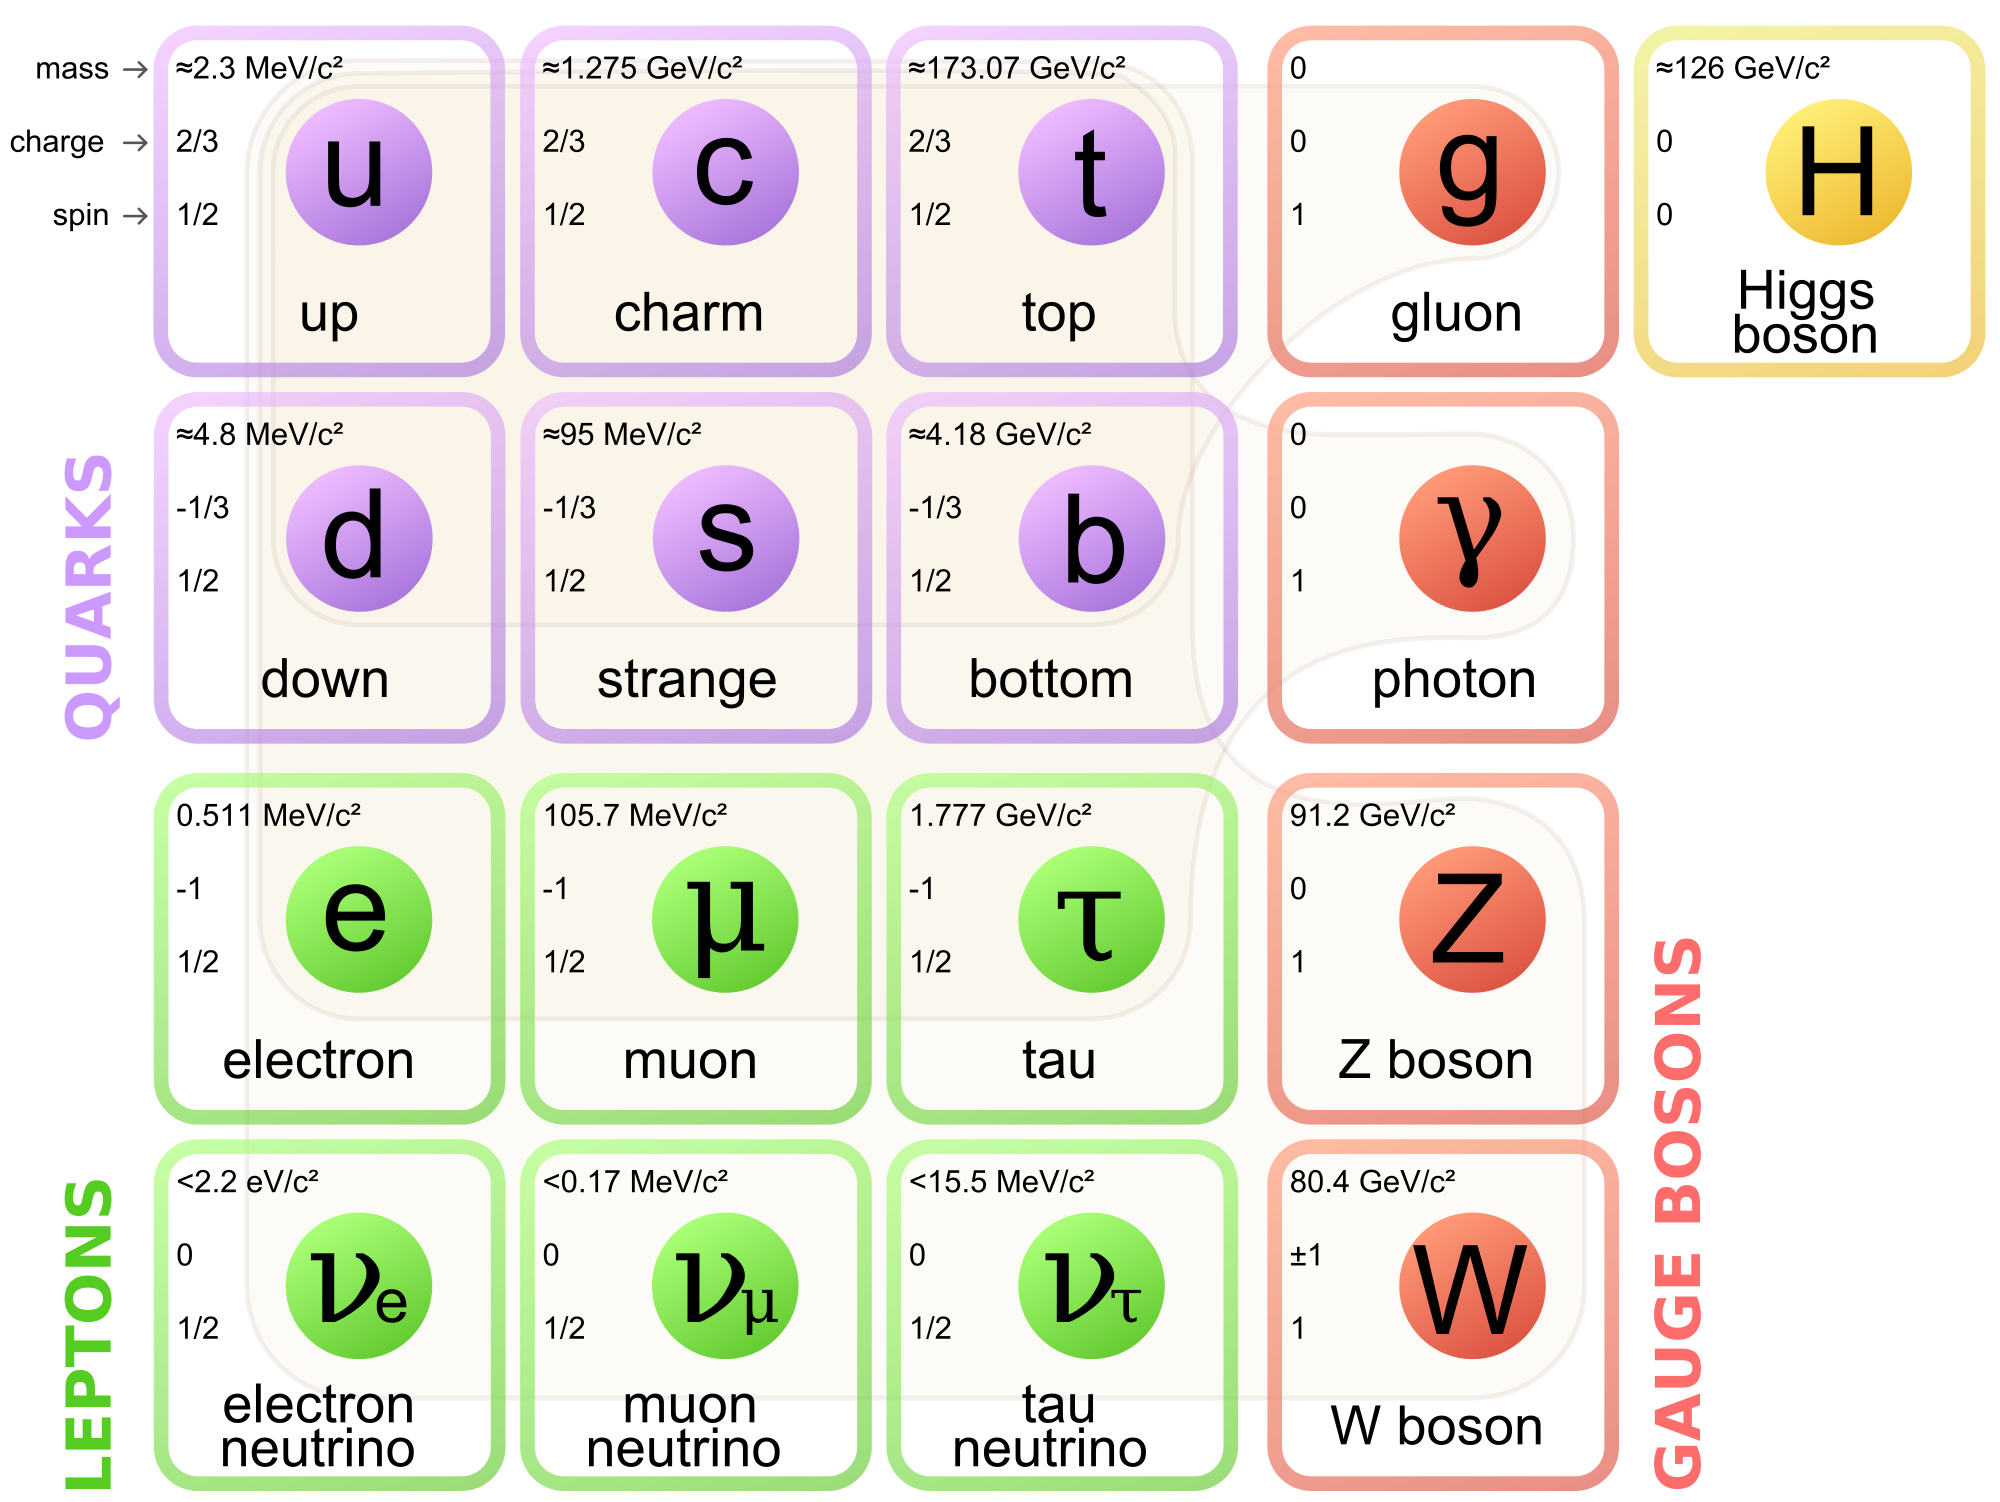
\includegraphics[width=\textwidth]{Chapter1/SM.png} 
  \caption{The system of fundamental particles of the SM. Figure from
    \cite{wiki:SMParticlesSource}}
  \label{fig:SMparticles}
\end{figure}

Quarks bind together to form hadrons and there are hundreds (?source?) of known
hadrons up to date. Theory describing the interaction between quarks is called
Quantum Chromodynamics (QCD) which key features will be discussed in this
chapter. The reasoning for quark existence and for the description their strong
interaction as $SU(3)$ gauge theory will be presented. Running coupling constant
will be discussed to split QCD into perturbative and non-perturbative regions -
two regions, where QCD has to use different mathematical approach for description of
strong interaction. Most of ideas presented here is overtaken from the following
textbook \cite{QCDTextbook}.

\section{Theoretical Ansatz}

In 1950s there have already been discovered tens of new hadrons thanks to new
particle accelerators and a lot of effort was exerted to categorize them. To each
particle there was except its mass assigned a series of quantum numbers
including isospin $T$ with its third component $T_3$, hypercharge $Y$,
electrical charge $Q$, strangeness $S$, baryon number $B$ and others. Soon it
was recognized, that there are some symmetries between these quantum numbers,
like Gell-Mann--Nishijima relation \cite{GellMannNishijima1,GellMannNishijima2}

\begin{equation}
  Q = T_3 + 1/2 Y \quad , \quad Y = B + S + \dots,
  \label{ex:GellMannNishijima}
\end{equation}
where dots denotes charm, bottomness and topness. 

\begin{table}
  \centering
  \begin{tabular}{|C{1cm}|C{1cm}|C{1cm}|C{1cm}|C{1cm}|C{1cm}|}
    \multicolumn{1}{c|}{} & $S$ & $Y$ & $T$ & $T_3$ & $Q$  \\
    \hline \hline
    $p$ & \multirow{2}{*}{0} & \multirow{2}{*}{1} & \multirow{2}{*}{1/2} & 1/2  & 1 \\
    $n$ &                    &                    &                      & -1/2 & 0 \\
    \hline                                                              
    $\Sigma^+$  & \multirow{4}{*}{-1} & \multirow{4}{*}{0} & \multirow{3}{*}{1} & 1  & 1  \\
    $\Sigma^0$  &                     &                    &                    & 0  & 0  \\
    $\Sigma^-$  &                     &                    &                    & -1 & -1 \\
    $\Lambda$   &                     &                    & 0                  & 0  & 0  \\
    \hline                                                              
    $\Xi^0$ & \multirow{2}{*}{-2} & \multirow{2}{*}{-1} & \multirow{2}{*}{1/2} & 1/2 & 0  \\
    $\Xi^-$ &                     &                     &                      &-1/2 & -1 \\
    \hline
  \end{tabular}
  \caption{Quantum numbers of selected hadrons known in 1950s. $S$ strangeness,
  $Y$ hypercharge, $T$ isospin, $T_3$ third component of isospin, $Q$ electrical
charge.}
  \label{tab:SelectedHadrons}
\end{table}


\begin{table}
  \centering
  \begin{tabular}{|C{1cm}|C{1cm}|C{1cm}|C{1cm}|C{1cm}|C{1cm}|}
    \multicolumn{1}{c|}{} & $S$ & $Y$ & $T$ & $T_3$ & $Q$  \\
    \hline \hline
    $u$ & \multirow{2}{*}{0} & \multirow{2}{*}{1/3} & \multirow{2}{*}{1/2} & 1/2
    & 2/3 \\
    $d$ &                    &                      &                      &
    -1/2 & \multirow{2}{*}{-1/3} \\
    $s$ & -1                 & -2/3                 & 0                    & 0    &  \\
    \hline                                                              
  \end{tabular}
  \caption{Quantum numbers of three quarks which existence was predicted by
    Gell-Mann and Zweig in 1964.}
  \label{tab:SelectedQuarks}
\end{table}


\begin{figure}[!ht]
  \centering
  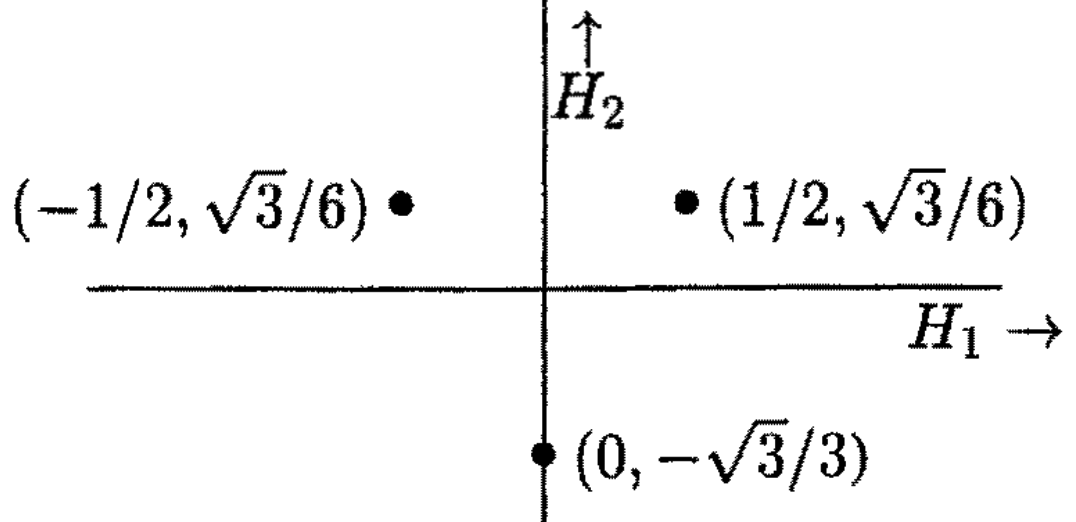
\includegraphics[width=0.5\textwidth]{Chapter1/Quark-triplet.png} 
  \caption{Eigenvalues of 3-dimensional representation of $\mathfrak{su}(3)$ Lie algebra. Figure
    from \cite{LieAlgebrasForParticlePhysicists}.}
  \label{fig:QuarkTriplet}
\end{figure}


\begin{figure}[!ht]
  \centering
  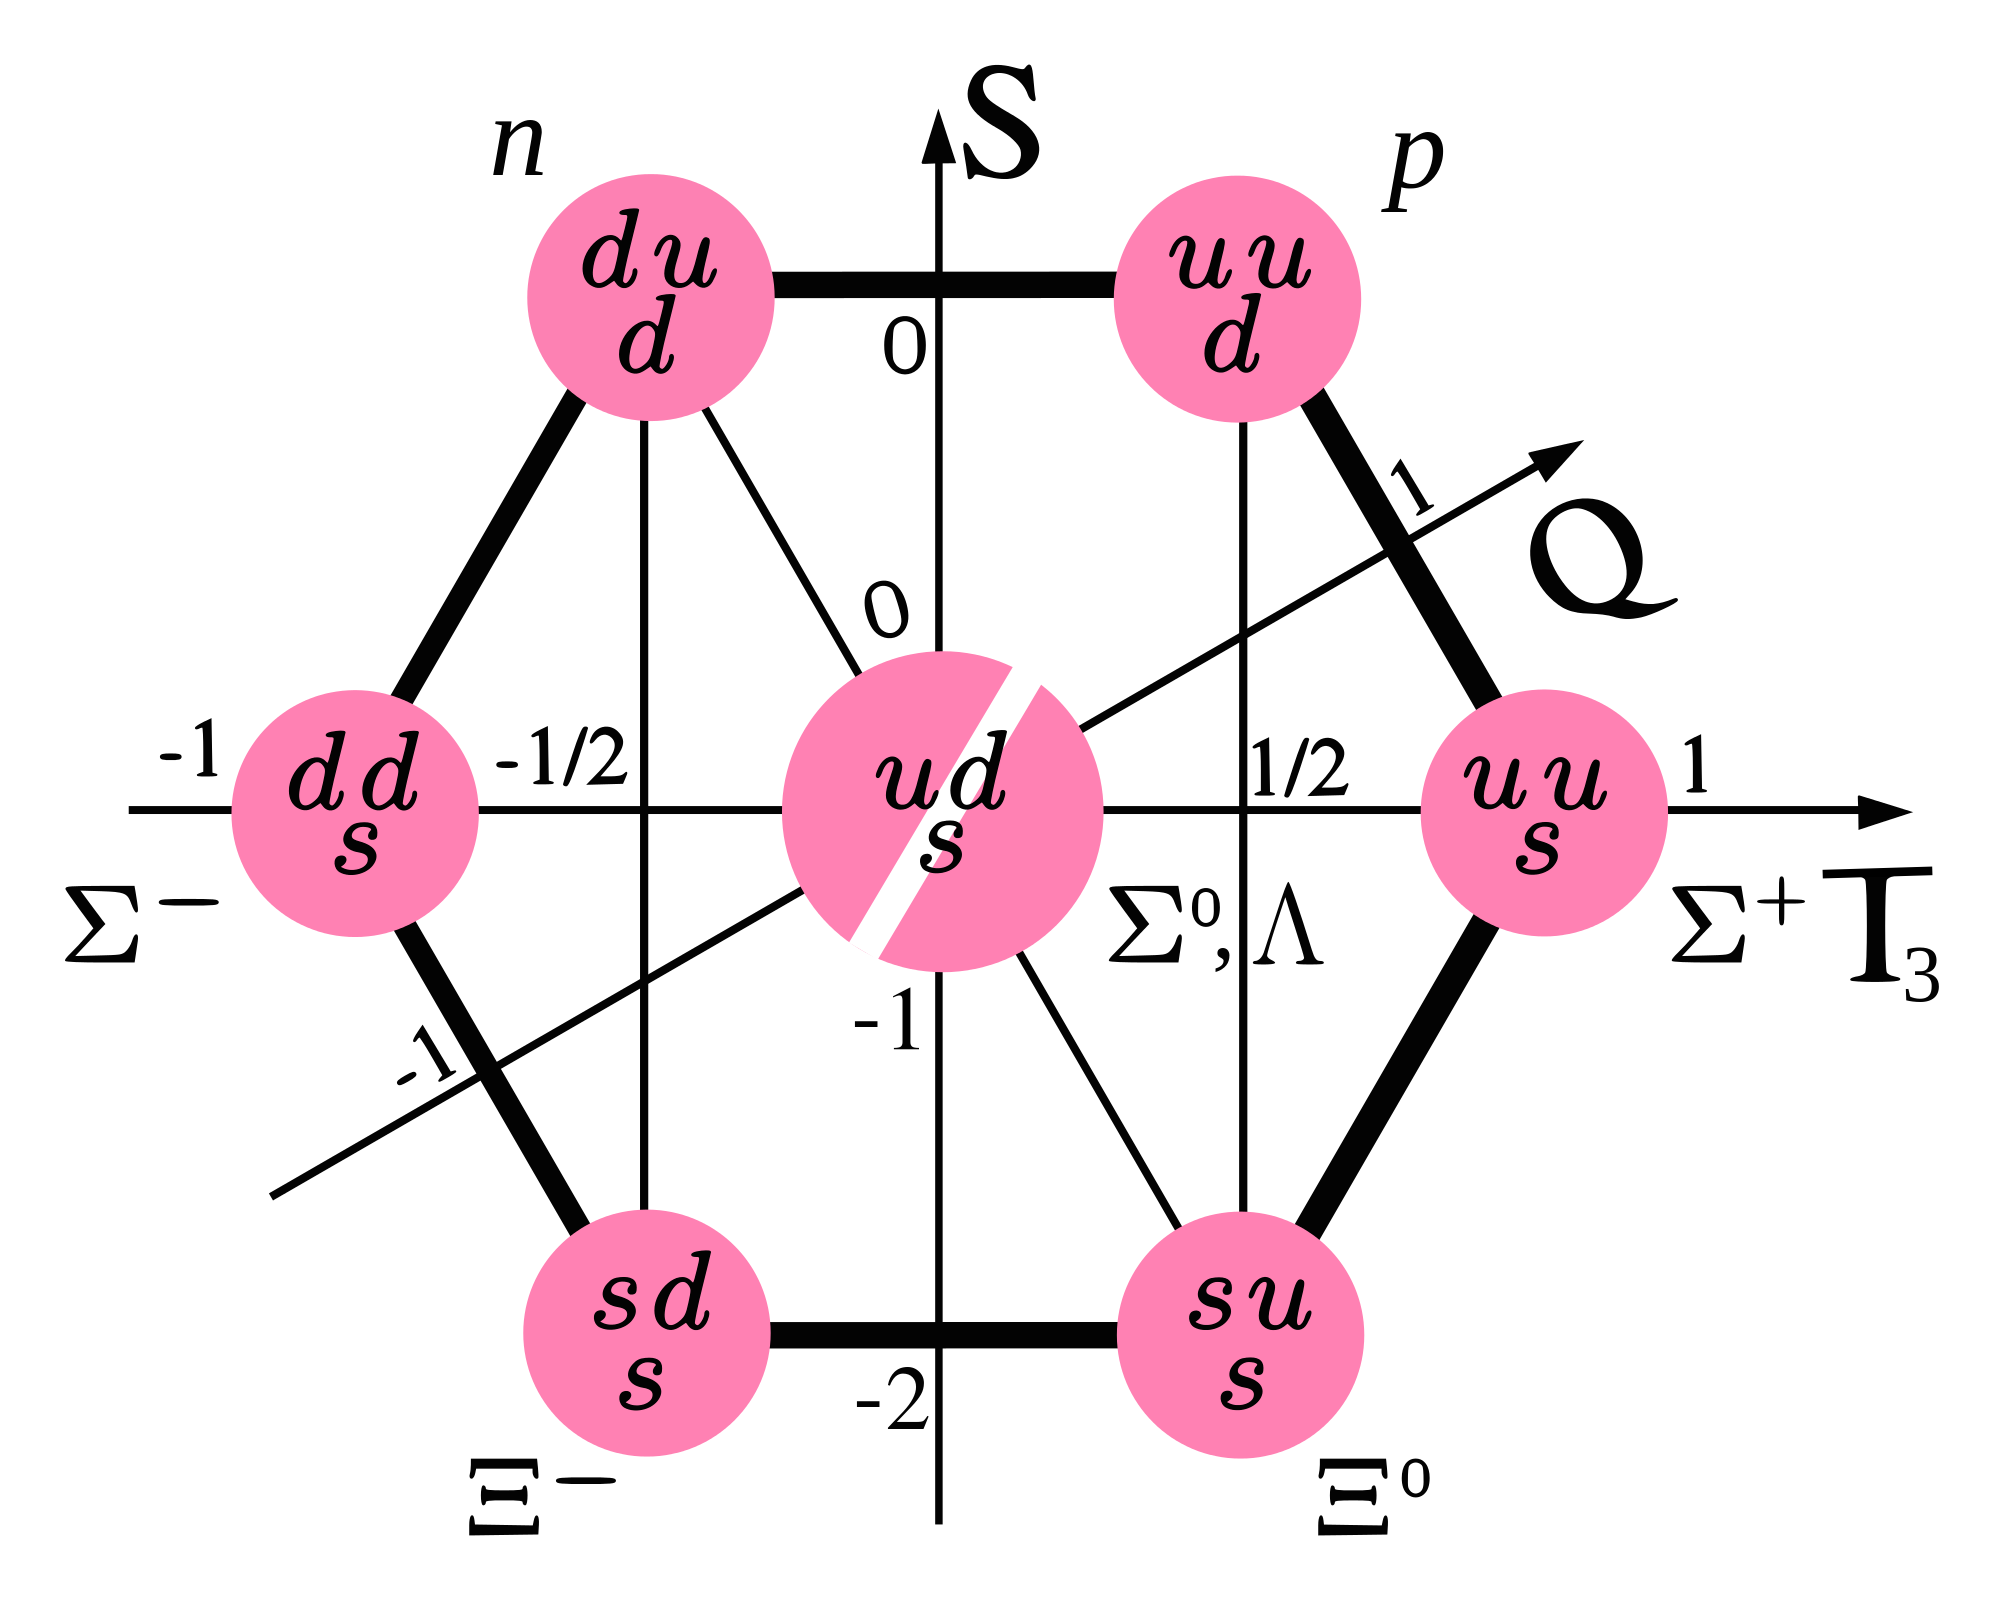
\includegraphics[width=0.5\textwidth]{Chapter1/Baryon-octet.png} 
  \caption{Baryonic octet encapsulating baryons from table
    \ref{tab:SelectedHadrons}. Figure from \cite{wiki:EightFoldWay}.}
  \label{fig:BaryonicOctet}
\end{figure}



\section{Experimental Ground}

\section{QCD as Gauge Theory}

\section{Perturbative QCD}

\section{Non-Perturbative QCD}


\chapter{QCD on ATLAS}

\chapter{ATLAS Detector}
\label{ch:intro}


%================================================================================
% Obrazky
%================================================================================
\clearpage
\listoffigures
\addcontentsline{toc}{chapter}{\listfigurename}


%================================================================================
% Tabulky
%================================================================================
\clearpage
\listoftables
\addcontentsline{toc}{chapter}{\listtablename}


%================================================================================
% Bibliografie
%================================================================================

\clearpage
\bibliographystyle{ieeetr}
\bibliography{bibliography}
\addcontentsline{toc}{chapter}{Bibliography}

\end{document}
